%------------------------------------------------------------------------------
\chapter{Implementation details}
\label{ch:implementation_details}

In this chapter we will explain how to use the shaders which have been implemented and the minor differences between the theoretical pipeline explained in Chapter~\ref{ch:methodology} and the actual software implementation.
An overview of the pipeline is shown in Figure~\ref{fig:pipeline_simplified}, note that modules in grey have not been implemented.

\begin{figure}[htbp!]
	\centering
	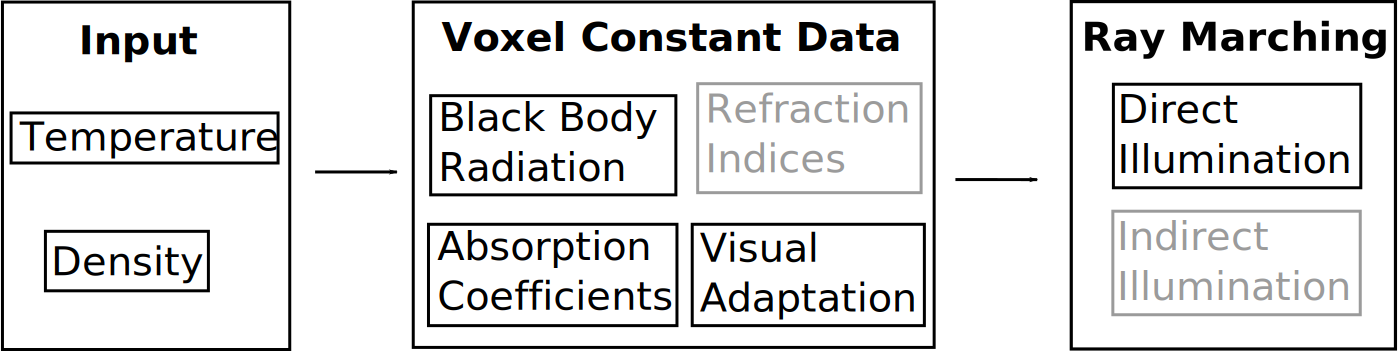
\includegraphics[width=\textwidth]{img/pipeline_simplified}
	\caption{An overview of the implemented fire rendering pipeline.}
	\label{fig:pipeline_simplified}
\end{figure}

\section{Application Overview}
\label{sec:application_overview}

The model chosen for our data is that of a three-dimensional voxel dataset, a cube in space is uniformly divided and a data value for each voxel.
This data is either a soot density estimate for the \textit{fire volume shader} or a temperature estimate for the \textit{fire light shader}.
Three file formats are supported, dense and sparse float voxel data is ASCII, and sparse binary RGBA values, as shown in Figure~\ref{fig:file_format}.
In the ASCII dense format, the file first line are three integers, separated by spaces, declaring the width, height and depth of the data, and $w \cdot h \cdot d$ lines with a single floating point values.
The ASCII sparse format, has two extra parameters in the first line, $c$ number of data points in the file and $b$ default value for any voxel that is not specified in the file.
Each data line has the $x,y,z$ coordinates and the data value separated by spaces.
The binary sparse format starts with a 4 byte integer declaring how many data points are in the file, each voxel has its coordinates $x,y,z$ as 4 bytes integers and a rgb alpha colour, where each channel is an 8 bytes floating point double value.
Values not included in the file are considered to be initialized to zero. 

\begin{figure}[htpb!]
        \centering
        \begin{subfigure}[t]{0.2\textwidth}
                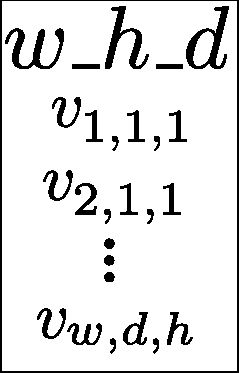
\includegraphics[width=\textwidth]{img/file_format_ascii_dense}
                \caption{ASCII dense (*.vol).}
                \label{fig:file_format_ascii_dense}
        \end{subfigure}%
        ~ %add desired spacing between images, e. g. ~, \quad, \qquad, \hfill etc.
          %(or a blank line to force the subfigure onto a new line)
        \begin{subfigure}[t]{0.3\textwidth}
                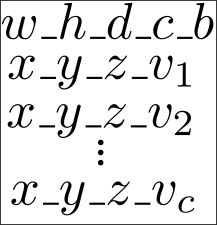
\includegraphics[width=\textwidth]{img/file_format_ascii_sparse}
                \caption{ASCII sparse (*.uintah).}
                \label{fig:file_format_ascii_sparse}
        \end{subfigure}
        ~ %add desired spacing between images, e. g. ~, \quad, \qquad, \hfill etc.
          %(or a blank line to force the subfigure onto a new line)
        \begin{subfigure}[t]{0.282\textwidth}
                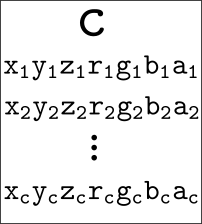
\includegraphics[width=\textwidth]{img/file_format_binary}
                \caption{Binary sparse (*.raw).}
                \label{fig:file_format_binary}
        \end{subfigure}
        \caption{Suported file formats, $\_$ represent the character space.}
        \label{fig:file_format}
\end{figure}

\section{\MentalRay Rendering Approach}
\label{sec:mental_ray_rendering_approach}

How mental ray shoots rays around and what is its paradigm.

\MentalRay approach to solving the rendering equation is based on path tracing, as shown in Figure~\ref{fig:mental_ray_model}, for each pixel in the camera view, an eye ray will be shot in the scene.
On an intersection with an object in the scene, its material shader will be called, this shader will shoot a light ray for each light in the scene, which in effects calls the light shader of the given light.
In order to compute the irradiance at the intersection point, the light shader will probably trace a shadow ray from the light to the intersection point.
Eventually, the material shader will compute the final colour with the information received from the light shader. 

\begin{figure}[htbp!]
\centering
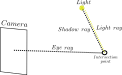
\includegraphics[width=0.8\textwidth]{img/mental_ray_model}
	\caption{\MentalRay simple ray casting example.}
	\label{fig:mental_ray_model}
\end{figure}

Under this assumptions, the steps required to solve the RTE, Equation~\ref{eq:rte_solution_paper}, are:

\begin{enumerate}
\item Shoot a ray from the eye into the scene
\item If the ray intersects the fire volume, perform ray marching in the volume
	\begin{enumerate}
	\item Compute direct illumination at the current point
		\begin{enumerate}
		\item Get initial radiance using black body radiation
		\item Attenuate with absorption coefficient
		\end{enumerate}
	\item Compute indirect illumination at the current point
		\begin{enumerate}
		\item Use phase function to get the scattered light distribution
		\end{enumerate}
	\item Advance to next point in ray marching
		\begin{enumerate}
		\item Change ray direction using refraction index
		\end{enumerate}	
	\end{enumerate}
\item Compute eye visual adaptation to fire colour
\end{enumerate}

Equation~\ref{eq:rte_solution_paper} provides a radiance value for the next march increment, however we want to compute the value at the ray intersection with the volume, i.e. at the ray origin.
So we need to rewrite the equation as

\begin{equation}
\begin{split}
L(\lambda, \x, \omegam) &= e^{\sigma_t(\lambda, \x) \deltax} L(\lambda, \x + \Delta\x, \omegam) +  \\
& (1 - e^{\sigma_t(\lambda, \x) \deltax} ) \frac{\sigma_a(\lambda, \x) L_e(\lxo) + \sigma_s(\lambda, \x) L_i(\lxo)}{\sigma_t(\lambda, \x)}.
\end{split}
\end{equation}

In fire phenomena the effect the scattered light in the final image is practically imperceptible~\cite{Pegoraro:2006}.
Exploiting the previous prior knowledge, the scattering contributions can be safely ignored by setting the coefficient $\sigma_s$ equal to zero, which simplifies the previous equation to

\begin{equation}
L(\lambda, \x, \omegam) = e^{\sigma_a(\lambda, \x) \deltax} L(\lambda, x + \Delta\x, \omegam) +  (1 - e^{\sigma_a(\lambda, \x) \deltax}) L_e(\lxo).
\end{equation}

A visual representation of the implications of the aforementioned simplification is shown in Figure~\ref{fig:ray_marching}.
Note that a single point light is used in the diagram to avoid clutter, yet in our implementation there is a point light located at the centre of each voxel whose temperature is high enough to be emissive.

\begin{figure}[htbp!]
	\centering
	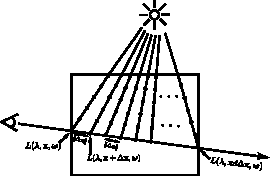
\includegraphics[width=0.8\textwidth]{img/ray_marching}
	\caption{Calculating the illumination values for samples along a ray.}
	\label{fig:ray_marching}
\end{figure}

\section{Shaders}
\label{sec:shaders}

Talk about things like which parts are written in parallel code, instance support, shader internal memory, sparse data, how the software escalates, memory consumption, Maya integration, spectrum to RGB integration, maybe more details about units for black body radiation and everything that was not explained before

\begin{figure}[htbp!]
\centering
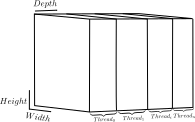
\includegraphics[width=0.5\textwidth]{img/voxel_thread_division}
	\caption{Voxel Dataset division of coefficients computation in threads.}
	\label{fig:voxel_dataset_threaded}
\end{figure}

\begin{figure}[htpb!]
        \centering
        \begin{subfigure}[b]{0.7\textwidth}
                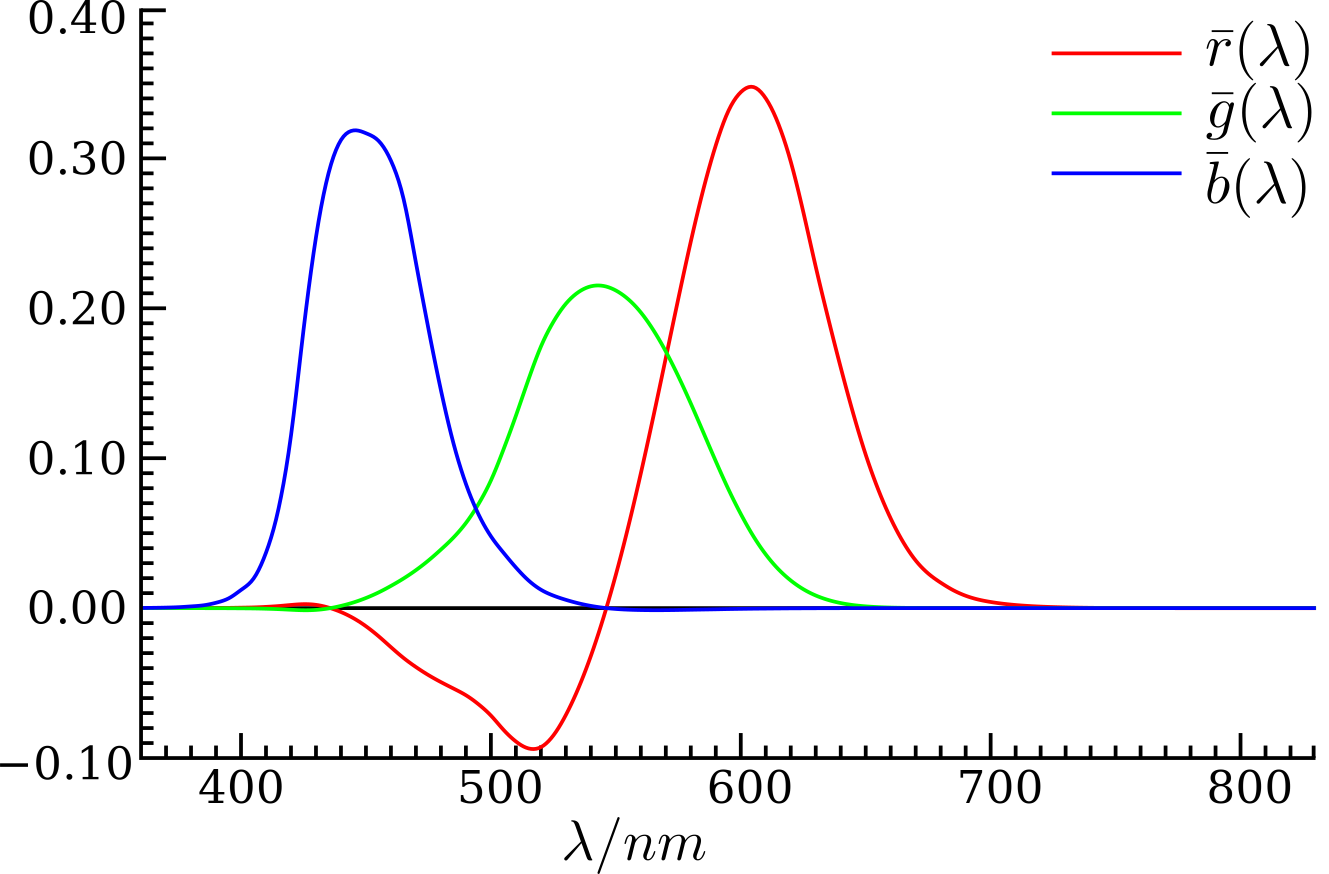
\includegraphics[width=\textwidth]{img/CIE_RGB}
                \caption{Spectral tristimulus values for CIE RGB~\cite{CIE_RGB}.}
                \label{fig:cie_rgb}
        \end{subfigure}%
        \quad %add desired spacing between images, e. g. ~, \quad, \qquad, \hfill etc.
          %(or a blank line to force the subfigure onto a new line)
        \begin{subfigure}[b]{0.7\textwidth}
                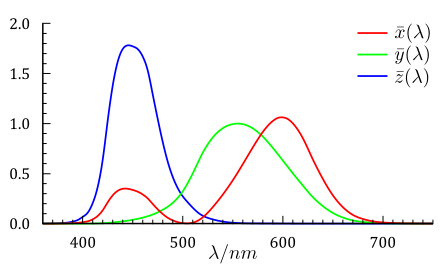
\includegraphics[width=\textwidth]{img/CIE_XYZ}
                \caption{Spectral tristimulus values for CIE XYZ~\cite{CIE_XYZ}.}
                \label{fig:cie_xyz}
        \end{subfigure}
        \caption{Colour matching curves for RGB and XYZ spaces.}
\end{figure}

In order to speed up the render time, all spectrum related computations are integrated to RGB coefficients.
Our spectrum class has a number of samples that can be set a compile time, 30 samples were used in all of our renderings.
To compute the absorption coefficients, Section~\ref{sec:absorption_coefficients}, data from Table~\ref{tb:soot_absorption_coefficients} is used.
Since, there is not enough data to cover the 30 spectrum coefficients, linear interpolation is used to be fill the missing values.
RGB coefficients are the standard colour representation used in computer screens, however not every colour visible by the human eye can be reproduced in the RGB space.
A further disadvantage, is that for certain colours negative values for the $\bar{r}(\lambda)$ coefficient are needed, as shown in Figure~\ref{fig:cie_rgb}.
The XYZ colour space is built using three sets of imaginary primaries, which have a series of favourable properties.
Any colour which can be seen by the human eye can be represented with some $x(\lambda)$, $y(\lambda)$, $z(\lambda)$ coefficients, the Y channel is equal to the photopic luminous efficiency function $V(\lambda)$, which models the variation of perceived brightness, and as shown in Figure~\ref{fig:cie_xyz}, the coefficients are always positive.

Given a Spectral Power Distribution (SPD) $S(\lambda)$, the $x$, $y$, $z$ coefficients for $S(\lambda)$ in the XYZ space are defined with respect to spectral matching curves $X(\lambda)$, $Y(\lambda)$ and $Z(\lambda)$, such that

\begin{equation}
\begin{split}
x &= \frac{1}{\int Y(\lambda) d\lambda} \int_\lambda S(\lambda) X(\lambda) d\lambda, \\
y &= \frac{1}{\int Y(\lambda) d\lambda} \int_\lambda S(\lambda) Y(\lambda) d\lambda, \\
z &= \frac{1}{\int Y(\lambda) d\lambda} \int_\lambda S(\lambda) Z(\lambda) d\lambda.
\end{split}
\end{equation}

The term $1 / \int Y(\lambda) d\lambda$ is added in each equation to act as a normalization factor for the colour brightness. 
As we are concerned with sampled values on a discrete domain, the integration for XYZ coefficients is approximated by a Rienmann sum

\begin{equation}
\begin{split}
x &\approx \frac{1}{\int Y(\lambda) d\lambda} \sum_i X_i c_i, \\
y &\approx \frac{1}{\int Y(\lambda) d\lambda} \sum_i Y_i c_i, \\
z &\approx \frac{1}{\int Y(\lambda) d\lambda} \sum_i Z_i c_i,
\end{split}
\end{equation}

where $c_i$ is the $i^{th}$ coefficient in the SPD, $X_i$ is area for the the corresponding sample range the $X(\lambda)$ curve and equivalently for $Y_i$ and $Z_i$.
Note that $1 / \left(\int Y(\lambda) d\lambda \right)$, $X_i$, $Y_i$ and $Z_i$ are constants and they can be precomputed for efficiency.
For the Rienmann sum, the area under the samples is approximated using piecewise linear interpolation.
The conversion from XYZ to RGB space is performed using

\begin{equation}
\begin{bmatrix}
r \\
g \\
b
\end{bmatrix}
 = 
\begin{bmatrix}
\int R(\lambda) X(\lambda) d\lambda & \int R(\lambda) Y(\lambda) d\lambda & \int R(\lambda) Z(\lambda) d\lambda \\
\int G(\lambda) X(\lambda) d\lambda & \int G(\lambda) Y(\lambda) d\lambda & \int G(\lambda) Z(\lambda) d\lambda \\
\int B(\lambda) X(\lambda) d\lambda & \int B(\lambda) Y(\lambda) d\lambda & \int B(\lambda) Z(\lambda) d\lambda
\end{bmatrix}
\begin{bmatrix}
x \\
y \\
z
\end{bmatrix},
\end{equation}

where $R(\lambda)$, $G(\lambda)$, $B(\lambda)$ are the spectral curves for the red, green and blue colours respectively.
Note that all the factors in the transformation matrix are constants and they can be precomputed for efficiency.

\subsection{Fire Volume Shader}
\label{sec:fire_volume_shader}

In order to achieve smoother rendering results, a trilinear interpolation is computed in each step in the ray-marching algorithm.
Computing the interpolation smoothed the shape of the flames and reduced the effects of outliers is the input data.
Tricubic interpolation was also considered, however it was discarded due to the significant increase in computational overhead.

The implementation of the eye visual adaptation to the colours in fire, described in Equation~\ref{eq:visual_adaptation} is performed as described in~\cite{Nguyen:2002}, which uses Von Kries model~\cite{Fairchild:2005} 

\begin{equation}
\begin{split}
\x_a &= \mathbf{M}^{-1} \mathbf{T}_w \mathbf{M} \x_i, \\
\mathbf{l}_{max} &= \mathbf{M} \mathbf{x}_{max}, \\
\mathbf{T}_w &= 
\begin{bmatrix}
1 / l_{max} & 0 & 0\\
0 & 1 / m_{max} & 0\\
0 & 0 & 1 / s_{max}\\
\end{bmatrix}, \\
\mathbf{M} &= 
\begin{bmatrix}
0.4002 & 0.7076 & -0.0808\\
-0.2263 & 1.1653 & 0.0457\\
0 & 0 & 0.9182\\
\end{bmatrix},
\end{split}
\end{equation}

where $\x_a = \left[ x_a, y_a, z_a \right]^{T}$ is a column vector with the XYZ adapted coefficients, $\mathbf{T}_w$ is the Von Kries transformation, $x_{max}$ are the coefficients for the maximum temperature present in the fire,  $\mathbf{l}_{max} = \left[ l_{max}, m_{max}, s_{max} \right]^{T}$ are the LMS coefficients of $x_{max}$, $\mathbf{M}$ is a XYZ to LMS transformation matrix and, $\x_i = \left[ x_i, y_i, z_i \right]^{T}$ is a column vector with the XYZ input coefficients.
The XYZ to LMS $\mathbf{M}$ matrix is a Hunt-Pointer-Estevez transformation, proposed by~\cite{Hunt:1985}, which has been normalized to the CIE Standard Illuminant D65.
The coefficients for $M^{-1}$ are not given in the CIE specification.
Given that $M$ is a small $3 \times 3$ matrix, the inversion can be performed with any of the standard methods, in our case the default algorithm in \Matlab \textit{inv()} function was used, and the result was hard-coded in the shader.
Solving the aforementioned equation in the XYZ space, instead of the RGB, will improve the quality of the final rendered image.

\subsection{Fire Light Shader}
\label{sec:fire_light_shader}


\subsection{Voxel Dataset Shader}
\label{sec:voxel_dataset_shader}

\subsection{Other}
\label{sec:other}

Talk about the maya command and matlab script